\PassOptionsToPackage{unicode=true}{hyperref} % options for packages loaded elsewhere
\PassOptionsToPackage{hyphens}{url}
%
\documentclass[12pt,]{report}
\usepackage{lmodern}
\usepackage{amssymb,amsmath}
\usepackage{ifxetex,ifluatex}
\usepackage{fixltx2e} % provides \textsubscript
\ifnum 0\ifxetex 1\fi\ifluatex 1\fi=0 % if pdftex
  \usepackage[T1]{fontenc}
  \usepackage[utf8]{inputenc}
  \usepackage{textcomp} % provides euro and other symbols
\else % if luatex or xelatex
  \usepackage{unicode-math}
  \defaultfontfeatures{Ligatures=TeX,Scale=MatchLowercase}
\fi
% use upquote if available, for straight quotes in verbatim environments
\IfFileExists{upquote.sty}{\usepackage{upquote}}{}
% use microtype if available
\IfFileExists{microtype.sty}{%
\usepackage[]{microtype}
\UseMicrotypeSet[protrusion]{basicmath} % disable protrusion for tt fonts
}{}
\IfFileExists{parskip.sty}{%
\usepackage{parskip}
}{% else
\setlength{\parindent}{0pt}
\setlength{\parskip}{6pt plus 2pt minus 1pt}
}
\usepackage{hyperref}
\hypersetup{
            pdftitle={Resumenes},
            pdfauthor={MALLQUI BAÑOS Ricardo Michel},
            pdfborder={0 0 0},
            breaklinks=true}
\urlstyle{same}  % don't use monospace font for urls
\usepackage{color}
\usepackage{fancyvrb}
\newcommand{\VerbBar}{|}
\newcommand{\VERB}{\Verb[commandchars=\\\{\}]}
\DefineVerbatimEnvironment{Highlighting}{Verbatim}{commandchars=\\\{\}}
% Add ',fontsize=\small' for more characters per line
\usepackage{framed}
\definecolor{shadecolor}{RGB}{248,248,248}
\newenvironment{Shaded}{\begin{snugshade}}{\end{snugshade}}
\newcommand{\AlertTok}[1]{\textcolor[rgb]{0.94,0.16,0.16}{#1}}
\newcommand{\AnnotationTok}[1]{\textcolor[rgb]{0.56,0.35,0.01}{\textbf{\textit{#1}}}}
\newcommand{\AttributeTok}[1]{\textcolor[rgb]{0.77,0.63,0.00}{#1}}
\newcommand{\BaseNTok}[1]{\textcolor[rgb]{0.00,0.00,0.81}{#1}}
\newcommand{\BuiltInTok}[1]{#1}
\newcommand{\CharTok}[1]{\textcolor[rgb]{0.31,0.60,0.02}{#1}}
\newcommand{\CommentTok}[1]{\textcolor[rgb]{0.56,0.35,0.01}{\textit{#1}}}
\newcommand{\CommentVarTok}[1]{\textcolor[rgb]{0.56,0.35,0.01}{\textbf{\textit{#1}}}}
\newcommand{\ConstantTok}[1]{\textcolor[rgb]{0.00,0.00,0.00}{#1}}
\newcommand{\ControlFlowTok}[1]{\textcolor[rgb]{0.13,0.29,0.53}{\textbf{#1}}}
\newcommand{\DataTypeTok}[1]{\textcolor[rgb]{0.13,0.29,0.53}{#1}}
\newcommand{\DecValTok}[1]{\textcolor[rgb]{0.00,0.00,0.81}{#1}}
\newcommand{\DocumentationTok}[1]{\textcolor[rgb]{0.56,0.35,0.01}{\textbf{\textit{#1}}}}
\newcommand{\ErrorTok}[1]{\textcolor[rgb]{0.64,0.00,0.00}{\textbf{#1}}}
\newcommand{\ExtensionTok}[1]{#1}
\newcommand{\FloatTok}[1]{\textcolor[rgb]{0.00,0.00,0.81}{#1}}
\newcommand{\FunctionTok}[1]{\textcolor[rgb]{0.00,0.00,0.00}{#1}}
\newcommand{\ImportTok}[1]{#1}
\newcommand{\InformationTok}[1]{\textcolor[rgb]{0.56,0.35,0.01}{\textbf{\textit{#1}}}}
\newcommand{\KeywordTok}[1]{\textcolor[rgb]{0.13,0.29,0.53}{\textbf{#1}}}
\newcommand{\NormalTok}[1]{#1}
\newcommand{\OperatorTok}[1]{\textcolor[rgb]{0.81,0.36,0.00}{\textbf{#1}}}
\newcommand{\OtherTok}[1]{\textcolor[rgb]{0.56,0.35,0.01}{#1}}
\newcommand{\PreprocessorTok}[1]{\textcolor[rgb]{0.56,0.35,0.01}{\textit{#1}}}
\newcommand{\RegionMarkerTok}[1]{#1}
\newcommand{\SpecialCharTok}[1]{\textcolor[rgb]{0.00,0.00,0.00}{#1}}
\newcommand{\SpecialStringTok}[1]{\textcolor[rgb]{0.31,0.60,0.02}{#1}}
\newcommand{\StringTok}[1]{\textcolor[rgb]{0.31,0.60,0.02}{#1}}
\newcommand{\VariableTok}[1]{\textcolor[rgb]{0.00,0.00,0.00}{#1}}
\newcommand{\VerbatimStringTok}[1]{\textcolor[rgb]{0.31,0.60,0.02}{#1}}
\newcommand{\WarningTok}[1]{\textcolor[rgb]{0.56,0.35,0.01}{\textbf{\textit{#1}}}}
\usepackage{longtable,booktabs}
% Fix footnotes in tables (requires footnote package)
\IfFileExists{footnote.sty}{\usepackage{footnote}\makesavenoteenv{longtable}}{}
\usepackage{graphicx,grffile}
\makeatletter
\def\maxwidth{\ifdim\Gin@nat@width>\linewidth\linewidth\else\Gin@nat@width\fi}
\def\maxheight{\ifdim\Gin@nat@height>\textheight\textheight\else\Gin@nat@height\fi}
\makeatother
% Scale images if necessary, so that they will not overflow the page
% margins by default, and it is still possible to overwrite the defaults
% using explicit options in \includegraphics[width, height, ...]{}
\setkeys{Gin}{width=\maxwidth,height=\maxheight,keepaspectratio}
\setlength{\emergencystretch}{3em}  % prevent overfull lines
\providecommand{\tightlist}{%
  \setlength{\itemsep}{0pt}\setlength{\parskip}{0pt}}
\setcounter{secnumdepth}{5}

% set default figure placement to htbp
\makeatletter
\def\fps@figure{htbp}
\makeatother

\usepackage{etoolbox}
\makeatletter
\providecommand{\subtitle}[1]{% add subtitle to \maketitle
  \apptocmd{\@title}{\par {\large #1 \par}}{}{}
}
\makeatother
\usepackage[scaled=0.92]{helvet}

\renewcommand{\rmdefault}{ptm}
%\usepackage{times}		
\usepackage{amsmath}		
\usepackage[lite,subscriptcorrection,slantedGreek,nofontinfo]{mtpro2}
\usepackage{booktabs}
\usepackage{enumitem}
\usepackage[a4paper]{geometry}
\geometry{verbose,tmargin=2.5cm,bmargin=2.5cm,lmargin=3cm,rmargin=2.5cm}
\setcounter{secnumdepth}{3}
\setcounter{tocdepth}{3}
\setlength{\parindent}{2.0em}
\usepackage{color}


\usepackage{titlesec}
\newcommand{\ww}{0.015em}
\titlespacing*{\chapter}
{0pt} {5em plus \ww minus \ww} {0em plus \ww minus \ww}
\titlespacing*{\section}
{0pt} {0em plus \ww minus \ww}{0em plus \ww minus \ww}
\titlespacing*{\subsection}
{0pt} {0em plus \ww minus \ww}{0em plus \ww minus \ww}
\titlespacing*{\subsubsection}
{0pt} {0em plus \ww minus \ww}{0em plus \ww minus \ww}
\titlespacing*{\paragraph} {0pt}{1.25ex plus 1ex minus .2ex}{2em}
\titlespacing*{\subparagraph} {\parindent}{3.25ex plus 1ex minus .2ex}{1em}
\titleformat*{\section}{\normalsize\bfseries}
\titleformat*{\subsection}{\normalsize\bfseries}
\setlength{\parskip}{0.5em plus \ww minus \ww}

\titleformat{\chapter}[display]
{\normalfont\normalsize\bfseries\centering}{Capítulo \thechapter}{0.0em}{\normalsize\bfseries}
%%%%%%%%%%%%%%%%%%%%%%%%%%
\usepackage{xpatch}%space equation
\xapptocmd\normalsize{%
	\abovedisplayskip=0.5em plus \ww minus \ww
	\abovedisplayshortskip=0.5em plus \ww minus \ww
	\belowdisplayskip=0.5em plus \ww minus \ww
	\belowdisplayshortskip=0.5em plus \ww minus \ww
}{}{}
%%%%%%%%%%%%%%%%%%%%%
%\setlength\intextsep{0.5em}% plus \ww minus \ww}
\setlist{topsep=0em plus \ww minus \ww, parsep=0.5em plus \ww minus \ww, itemsep=0em} 

\setcounter{topnumber}{2}
\setcounter{bottomnumber}{2}
\setcounter{totalnumber}{4}
\renewcommand{\topfraction}{0.85}
\renewcommand{\bottomfraction}{0.85}
\renewcommand{\textfraction}{0.5}
\renewcommand{\floatpagefraction}{0.7}



\newcommand{\N}{\mathds{N}}
\newcommand{\R}{\mathds{R}}
\newcommand{\CC}{\mathds{C}}
\newcommand{\I}{\mathds{I}}
\newcommand{\f}{\mathds{f}}
\newcommand{\X}{\mathds{X}}
\newcommand{\D}{\mathds{D}}
\newcommand{\Z}{\mathds{Z}}
\newcommand{\Q}{\mathds{Q}}

\newcommand{\Ee}{\mathcal{E}}
\newcommand{\Pp}{\mathcal{P}}
\newcommand{\Ll}{\mathcal{L}}
\newcommand{\Hh}{\mathcal{H}}
\newcommand{\Cc}{\mathcal{C}}

\newcommand{\norm}[1]{\left\Vert#1\right\Vert}
\newcommand{\abs}[1]{\left\vert#1\right\vert}
\newcommand{\set}[1]{\left\{#1\right\}}
\newcommand{\seq}[1]{\left<#1\right>}
\newcommand{\co}[1]{\left[#1\right]}
\newcommand{\cc}[1]{\left(#1\right)}
% https://github.com/rstudio/rmarkdown/issues/337
\let\rmarkdownfootnote\footnote%
\def\footnote{\protect\rmarkdownfootnote}

% https://github.com/rstudio/rmarkdown/pull/252
\usepackage{titling}
\setlength{\droptitle}{-2em}

\pretitle{\vspace{\droptitle}\centering\huge}
\posttitle{\par}

\preauthor{\centering\large\emph}
\postauthor{\par}

\predate{\centering\large\emph}
\postdate{\par}
\usepackage[]{natbib}
\bibliographystyle{apalike}

\title{Resumenes}
\author{MALLQUI BAÑOS Ricardo Michel}
\date{2020-02-19}

\begin{document}
\maketitle

{
\setcounter{tocdepth}{1}
\tableofcontents
}
\hypertarget{prerequisites}{%
\chapter{Prerequisites}\label{prerequisites}}

\hypertarget{datos}{%
\section{Datos}\label{datos}}

Sean los datos que se prosiguen

\begin{itemize}
\tightlist
\item
  www
\item
  wwwww
\end{itemize}

\hypertarget{ff}{%
\subsection{ff}\label{ff}}

WWWW fff
WWWW wwwww

\hypertarget{ff-1}{%
\subsection{ff}\label{ff-1}}

This is a \emph{sample} book written in \textbf{Markdown}. You can use anything that Pandoc's Markdown supports, e.g., a math equation \(a^2 + b^2 = c^2_c\).

The \textbf{bookdown} package can be installed from CRAN or Github:

\begin{Shaded}
\begin{Highlighting}[]
\KeywordTok{install.packages}\NormalTok{(}\StringTok{"bookdown"}\NormalTok{)}
\CommentTok{# or the development version}
\CommentTok{# devtools::install_github("rstudio/bookdown")}
\end{Highlighting}
\end{Shaded}

Remember each Rmd file contains one and only one chapter, and a chapter is defined by the first-level heading .

To compile this example to PDF, you need XeLaTeX. You are recommended to install TinyTeX (which includes XeLaTeX): \url{https://yihui.org/tinytex/}.

\hypertarget{acciones}{%
\section{Acciones}\label{acciones}}

Sean los datos \emph{emph} \textbf{\emph{real}} \textbf{Entonces}

\hypertarget{intro}{%
\chapter{Introduction}\label{intro}}

You can label chapter and section titles using after them, e.g., we can reference Chapter \ref{literature}. If you do not manually label them, there will be automatic labels anyway, e.g., Chapter \ref{methods}.

Figures and tables with captions will be placed in and environments, respectively.

\begin{Shaded}
\begin{Highlighting}[]
\KeywordTok{par}\NormalTok{(}\DataTypeTok{mar =} \KeywordTok{c}\NormalTok{(}\DecValTok{4}\NormalTok{, }\DecValTok{4}\NormalTok{, }\FloatTok{.1}\NormalTok{, }\FloatTok{.1}\NormalTok{))}
\KeywordTok{plot}\NormalTok{(pressure, }\DataTypeTok{type =} \StringTok{'b'}\NormalTok{, }\DataTypeTok{pch =} \DecValTok{19}\NormalTok{)}
\end{Highlighting}
\end{Shaded}

\begin{figure}

{\centering 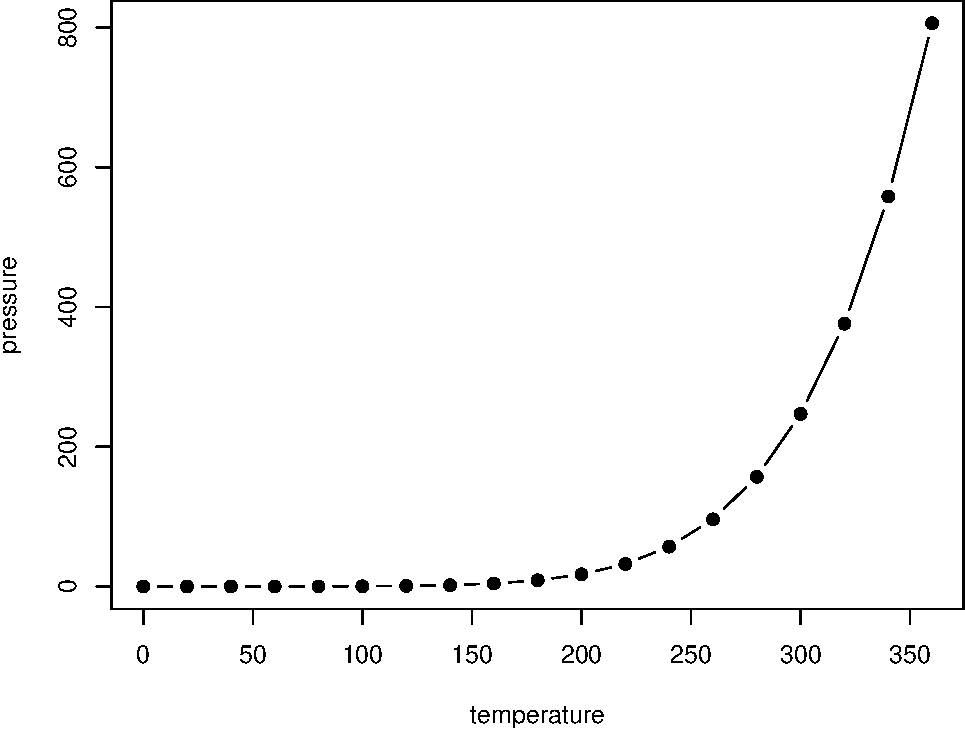
\includegraphics[width=0.8\linewidth]{Programacion_files/figure-latex/nice-fig-1} 

}

\caption{Here is a nice figure!}\label{fig:nice-fig}
\end{figure}

Reference a figure by its code chunk label with the prefix, e.g., see Figure \ref{fig:nice-fig}. Similarly, you can reference tables generated from \texttt{knitr::kable()}, e.g., see Table \ref{tab:nice-tab}.

\begin{Shaded}
\begin{Highlighting}[]
\NormalTok{knitr}\OperatorTok{::}\KeywordTok{kable}\NormalTok{(}
  \KeywordTok{head}\NormalTok{(iris, }\DecValTok{20}\NormalTok{), }\DataTypeTok{caption =} \StringTok{'Here is a nice table!'}\NormalTok{,}
  \DataTypeTok{booktabs =} \OtherTok{TRUE}
\NormalTok{)}
\end{Highlighting}
\end{Shaded}

\begin{table}

\caption{\label{tab:nice-tab}Here is a nice table!}
\centering
\begin{tabular}[t]{rrrrl}
\toprule
Sepal.Length & Sepal.Width & Petal.Length & Petal.Width & Species\\
\midrule
5.1 & 3.5 & 1.4 & 0.2 & setosa\\
4.9 & 3.0 & 1.4 & 0.2 & setosa\\
4.7 & 3.2 & 1.3 & 0.2 & setosa\\
4.6 & 3.1 & 1.5 & 0.2 & setosa\\
5.0 & 3.6 & 1.4 & 0.2 & setosa\\
\addlinespace
5.4 & 3.9 & 1.7 & 0.4 & setosa\\
4.6 & 3.4 & 1.4 & 0.3 & setosa\\
5.0 & 3.4 & 1.5 & 0.2 & setosa\\
4.4 & 2.9 & 1.4 & 0.2 & setosa\\
4.9 & 3.1 & 1.5 & 0.1 & setosa\\
\addlinespace
5.4 & 3.7 & 1.5 & 0.2 & setosa\\
4.8 & 3.4 & 1.6 & 0.2 & setosa\\
4.8 & 3.0 & 1.4 & 0.1 & setosa\\
4.3 & 3.0 & 1.1 & 0.1 & setosa\\
5.8 & 4.0 & 1.2 & 0.2 & setosa\\
\addlinespace
5.7 & 4.4 & 1.5 & 0.4 & setosa\\
5.4 & 3.9 & 1.3 & 0.4 & setosa\\
5.1 & 3.5 & 1.4 & 0.3 & setosa\\
5.7 & 3.8 & 1.7 & 0.3 & setosa\\
5.1 & 3.8 & 1.5 & 0.3 & setosa\\
\bottomrule
\end{tabular}
\end{table}

You can write citations, too. For example, we are using the \textbf{bookdown} package \citep{R-bookdown} in this sample book, which was built on top of R Markdown and \textbf{knitr} \citep{xie2015}.

\hypertarget{literature}{%
\chapter{Literature}\label{literature}}

Here is a review of existing methods.

\hypertarget{methods}{%
\chapter{Methods}\label{methods}}

We describe our methods in this chapter.

\hypertarget{applications}{%
\chapter{Applications}\label{applications}}

Some \emph{significant} applications are demonstrated in this chapter.

\hypertarget{example-one}{%
\section{Example one}\label{example-one}}

\hypertarget{example-two}{%
\section{Example two}\label{example-two}}

\hypertarget{final-words}{%
\chapter{Final Words}\label{final-words}}

\begin{enumerate}
\def\labelenumi{\arabic{enumi}.}
\item
  La circunferencia \(\mathcal{C}=(x-3)^2+()y-3^2=25\) es tangente a una parábola \(\mathcal{P}\) en \(P_0=(x_0,y_0)\), \(y>7\). La recta \(\mathcal{L}:4x-3y+12=0\) es normal a \(\mathcal{P}\) y \(\mathcal{C}\) en \(P_0\) y corta al eje focal de \(\mathcal{P}\) en el punto \(R\) foco de \(\mathcal{P}\). Si \(\left|\vec{C_0P_0}\right|=\left|\vec{P_0R}\right|\) y si la distnacia \(d[P_0;eje focal]=4\), hallar la ecuacion de la parabola \(\mathcal{P}\). \(C_0\) es el centro de la circunferencia y la absisa del vértice es menor que 6.
\item
  Los puntos \(A=(60,13)\) y \(B=(-4,61)\) estan sobre una parábola \(\mathcal{P}\) además son simétricos con recpecto al eje focal. Desde un punto \(Q\) sobre el eje focal se traza un recta tangente a \(\mathcal{P}\) que pasa por \(B,\) hallar la ecuación de \(\mathcal{P}\) y las ecuaciones de las rectas tangentes trazadas desde \(Q\).
\end{enumerate}

Ya que \(A\) y \(B\) son simétricas entonces \(P_0=\frac{A+B}{2}=(28,37) \in \mathcal{L}_F\) donde \(\mathcal{L}_F\) es el eje focal paralelo al vector \(\vec{AB}^\perp=(B-A)^\perp=(-64,48)\parallel(-4,3)=\vec{v}_L\) es decir \(\vec{v}_F\) y \(P_0\) nos genera la ecuación del eje focal \(\mathcal{L}_F:4x+3y=1\). De otro lado dado el punto \(Q=(20,x)\in\mathcal{L}_F\) que al reemplazarlo en la recta del eje focal nos genera \(x=-27\) de donde \(Q=(20,-27)\) ademas el vértice de la parabola es \(V=\frac{Q+P_0}{2}=(4,5)\) por propiedad.

Con el objetivo de hallar el valor de \(\rho\) en la ecuación \(y'^2=4\rho x'\) se halla las coordenadas de \(B\) en el nuevo sistema de coordenadas centrada en \(V\) con vector director \(\vec{u}=\frac{(3,4)}{5}\), haciendo uso de la relación \[(x,y)=V+x'\vec{u}+y'\vec{u}^\perp\] se obtiene \(x'=\left[B-V\right]\vec{u}=40\) y \(y'=\left[B-V\right]\vec{u}^\perp=40\) por tanto reemplazando \(B=(-4,61)=(40,40)'\) en \(y'^2=4\rho x'\) se tiene que \(\rho=10\)

Los vectores directores de las rectas tangentes en el sistema \(x'y'\) son \((2,1)\) y \((2,-1)\) respectivamente por tanto sus ecuaciones son \(\mathcal{L}_A: 2y'=x'+40\) y \(\mathcal{L}_B=-2y'=x'+40\) estas ecuaciones en el sistema original con \(x'=\left[(x,y)-(4,5)\right]\frac{(3,4)}{5}\) y \(y'=\left[(x,y)-(4,5)\right]\frac{(-4,3)}{5}\) reemplazadas resultan \(\mathcal{L}_A:2y-11x-166=0\) y \(\mathcal{L}_B:5x-10y-170=0\)

\begin{enumerate}
\def\labelenumi{\arabic{enumi}.}
\tightlist
\item
  ww
\end{enumerate}

\bibliography{book.bib,packages.bib}

\end{document}
